\section{Preliminaries}
\label{sec:model}

The vocabulary used throughout this document is described in the Glossary \cite{glossary}.
The reader is assumed to be familiar with the terminology defined there.
\jorge{Despite this not, the vocabulary seems to be defined throughout the body. If we're defining in the body anyway, the appendix seems redundant -- this isn't a book.}

% \subsection{Computation and failure model}

% We model \ipc as a distributed (``message-passing") system consisting of \emph{processes} that communicate by exchanging \emph{messages}%
% \footnote{Network messages are not to be confused with Filecoin actor messages, to which this document refers as transactions.}
% over a network. 
% In practice, a process is a program running on a computer, having some state, and reacting to external events and messages received over a communication network.
% We describe processes as exemplified in \Cref{alg:process-definition}.

% \begin{algorithm}[H]
% \footnotesize
% \caption{Process definition.}\label{alg:process-definition}
%   \DontPrintSemicolon
%   \SetKwProg{Component}{$\blacktriangleright$ \bf}{:}{\KwRet}
%   \SetKwFor{UponKW}{upon}{do}{fintq}
%   \SetKw{Trigger}{trigger}
%   variableA = initial value\\
%   variableB = initial value\\ \jorge{this is kind of a weird notation, as you can't tell whether you're defining a new variable or just assigning a new value}
%   ...\\
%   \Component{process}{
%      \UponKW{event(params...)}{
%        \tcp{Logic to execute atomically}
%      }
%      \UponKW{event(params...)}{
%        \tcp{Logic to execute atomically}
%      }
%      ...
% }
% \end{algorithm}

% A process that performs all the steps exactly as prescribed by the protocols in which it is participating is \emph{correct}.
% A process that stops performing any steps (i.e., \emph{crashes}) or that deviates from the prescribed protocols in any way is \emph{faulty}.
% If a process is correct or may only fail by crashing, it is \emph{benign}.
% A non-benign process is \emph{malicious}.
% \matej{We can remove terms we end up not using...}

% In general, faulty processes can be malicious (Byzantine): we do not put any restrictions on their behavior, except being computationally bounded and, thus, unable to subvert standard cryptographic primitives, such as forging signatures or inverting secure hash functions.
% If the implementation of some component in our design requires additional assumptions on the behavior of faulty processes, they will be stated explicitly.
% % We do not make a general statement about the fault tolerance of \ipc as a system, as to how many faulty processes the system can sustain.
% % This depends on the final implementation of its components.

% We use the term \emph{participant} to describe an entity participating in the system that controls one or more processes.
% All processes controlled by one participant are assumed to be in the same trust domain, that is, they assume one another's correctness.
% For example, a participant in the child subnet will probably run multiple processes:
% one for participating in the child subnet (child replica),
% one for participating in the parent subnet (parent replica),
% and one that processes the information from the two replicas and submits transactions accordingly (\ipc agent).
% We precisely define the replicas and the \ipc agent (all of them being processes) in \Cref{sec:components,sec:smr}.
% The \ipc agent of a participant always assumes that the information it receives from "its own" child replica is correct.
% However, messages received from another participant's replica or \ipc agent are seen as potentially malicious.

% The synchrony assumptions may vary between different components of \ipc.
% We thus state those assumptions whenever necessary, when describing concrete implementations of \ipc components.

% \subsection{State machine replication (SMR) and \actors}
% \label{sec:smr}

% \paragraph{SMR and replicated state.}
% A \emph{state machine replication (SMR) system}%
% is a system consisting of processes called \emph{replicas}, each of which locally stores a copy of (or at least has access to) \emph{replicated state}
% that it updates over time by applying a sequence of \emph{transactions} to it. 
% \jorge{it's not objectively wrong, but not a huge fan of defining replicas now, after they were mentioned several times}
% Without specifying the details, we assume that any process can \emph{submit} a transaction to an SMR system (we call such a process an \emph{SMR client})
% and that this transaction will eventually be ordered and applied to the replicated state.
% We call an SMR system that is part of \ipc a \emph{subnet}.

% An SMR system guarantees to each correct replica that, after applying $n$ transactions to its local copy of the replicated state,
% the latter will be identical to any other correct replicas' copy of the replicated state after applying $n$ transactions.
% The replicas achieve this by executing an \emph{ordering protocol} to agree on a common sequence of transactions to apply to the replicated state.

% Note that replicas do not necessarily all hold the same replicated state at any instant of real time,
% since each replica might be processing transactions at a different time.
% In this context, there is no such thing as “the current replicated state of the SMR system”.
% There is only the current replicated state of a single replica.
% The replicated state of the system is only an abstract, logical construct
% useful for reasoning about transitions from one replicated state to another,
% happening at individual replicas by applying transactions (at different real times).
% When referring to a “current” replicated state, we mean the state resulting from the application of a certain number of transactions to the initial state.

% \paragraph{Actors.}
% The replicated state of an SMR system can be logically subdivided into multiple \emph{\actors}.
% A \actor is a portion of the replicated state with well-defined semantics.
% It defines the logic that a replica needs to execute when applying transactions and the new state that results from it.

% We model a \actor as a logical object in the replicated state that contains arbitrary variables representing its state.
% Its associated logic reacts to \emph{events} triggered by (1) the application of transactions or (2) the execution of other (or even own) actor logic. \jorge{why "even own"? why is that more surprising than foreign actor logic?}
% We describe actors as exemplified in \Cref{alg:actor-definition}. \jorge{Is it a definition or an example?}


% \begin{algorithm}[H]
% \footnotesize
% \caption{\actor definition}\label{alg:actor-definition}
%   \DontPrintSemicolon
%   \SetKwProg{Component}{$\blacktriangleright$ \bf}{:}{\KwRet}
%   \SetKwFor{UponKW}{}{}{fintq}
%   \SetKw{Trigger}{trigger}
%   variable = initial value\\
%   variable = initial value\\
%   ...\\
%   \Component{\actor name}{
%      \UponKW{Function(params...)}{
%        \tcp{Logic to execute}
%      }
%      \UponKW{Function(params...)}{
%        \tcp{Logic to execute}
%      }
%   }
% \end{algorithm}
% While \emph{process} denotes an instance of a program running on some physical machine,
% \actors are an abstraction over the replicated state of an SMR system and their logic is being executed by all its replicas.
% While a process can submit a transaction to an SMR system, a \actor cannot.

\paragraph{Abstractions.}
In this document, we reason in terms of subnets, actors, accounts, users, and \ipc agents (see Glossary \cite{glossary}]).
While a subnet consists of multiple replicas, we treat it as one entity maintaining a common abstraction of a replicated state
that can only be modified through transactions submitted either by a users or by an \ipc agent.
We abstract away the concrete mechanism of transaction submission and execution, as it is specific to the implementation of each particular subnet.

\paragraph{Interaction between subnets.}
In \ipc, the replicated state of one subnet must react to (changes in) the replicated state of another subnet.
As the replicated state of every subnet is distributed among its replicas and evolves independently of other subnets,
we must establish a mechanism for interactions between the states of subnets.
In particular, we must explicitly link the two replicated states of two subnets.
More precisely, for any interaction between two subnets (\subnetName{A} and \subnetName{B}), define block heights $h_\subnetName{A}$ and $h_\subnetName{B}$,
such that \subnetName{A}'s replicated state at height $h_\subnetName{A}$ considers \subnetName{B}'s replicated state to have evolved exactly until $h_\subnetName{B}$.

\paragraph{\pofsFull.}
To enable interaction between subnets, we define a \emph{\pofFull (\pof)} to be data that proves that a subnet definitively reached a certain replicated state.
Regardless of the subnet's ordering protocol's approach to finality (e.g., immediate finality for classic BFT protocols, or probabilistic finality in PoW-based systems),
a \pof convinces the proof's verifier that the replicated state the \pof refers to will not be rolled back.
For example, for a subnet using a BFT-style ordering protocol, a quorum of signatures produced by its replicas can constitute a \pof.
This helps us establish the above-mentioned link between the replicated states of two subnets.
If a \pof is associated with subnet \subnetName{A}'s replicated state at $h_\subnetName{A}$,
and \pof is included in subnet \subnetName{B}'s replicated state at height $h_\subnetName{B}$,
then subnet \subnetName{B}'s replicated logic will consider all \subnetName{A}'s state changes up to $h_\subnetName{A}$
to have occurred at \subnetName{B}'s height $h_\subnetName{B}$.
We denote by \pof\unskip(\tx{tx}) the proof that a subnet reached a state in which transaction \tx{tx} already has been applied.

\paragraph{\ipc agent and actors.}
For inter-subnet communication, \ipc relies on two special types of actors (the \gwFull (\gw) and the \saFull (\sa)) and one special type of process (the \ipc Agent).
In a nutshell, their functions are as follows.
\begin{enumerate}
    \item The \gw is an actor that contains all \ipc-related information and logic associated with a subnet that needs to be replicated \emph{in the subnet itself}.
    \item The \sa is the \gw's parent-side counterpart, i.e., it is an actor in a parent subnet's replicated state,
    containing all the data and logic associated with a particular child subnet (we say the \sa ``governs'' that child subnet).
    \item Finally, the \ipc agent is a process that mediates the communication between a parent and a child.
    It has access to the replicated states of both subnets and acts as an SMR client of both.
    When the replicated state of subnet \subnetName{A} indicates the need to communicate with subnet \subnetName{B},
    the \ipc agent constructs a \pof for \subnetName{A}'s replicated state and submits it as a transaction to \subnetName{B}.
\end{enumerate}
The interaction between subnets through \ipc agents is depicted in \cref{fig:interfaces}.

\begin{figure}[ht]
     \centering
     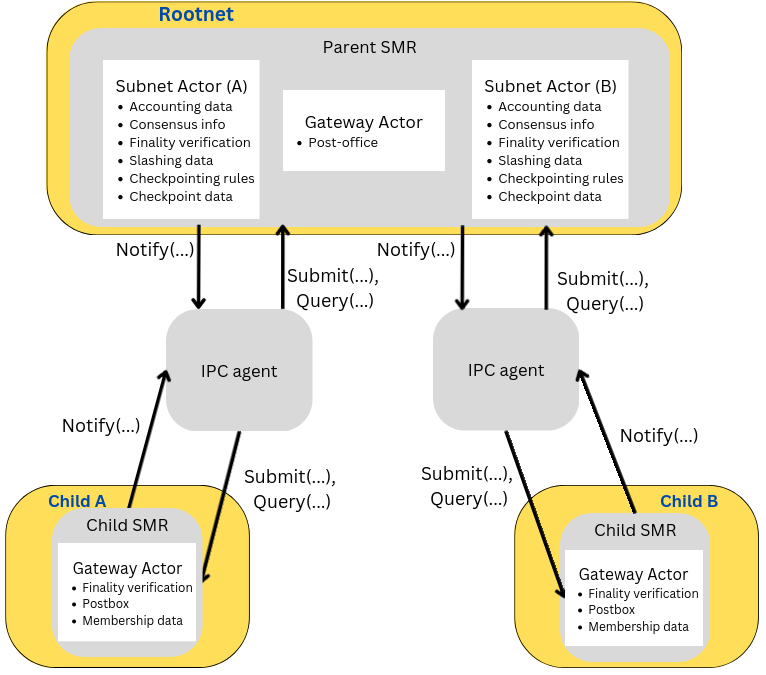
\includegraphics[width=0.75\textwidth]{compsintf-2subnets}
     \caption{The basic \ipc components and their interfaces in an example with one parent and 2 child subnets (A and B). \TODO{Update figure to be consistent with new notation.}}
     \label{fig:interfaces}
 \end{figure}

\paragraph{Naming subnets.}
We assign each subnet a name that is unique among all the children of the same parent.
Similarly to the notation used in a file system, the name of a child subnet is always prefixed by the name of its parent.
For example, subnets \subnetName{P/C} and \subnetName{P/D} would both be children of subnet \subnetName{P}.

\paragraph{Notation.} We refer to an account \accountName{a} in the replicated state of subnet \subnetName{S} as \subnetName{S}.\accountName{a}.
To denote a function of an actor in the replicated state of a subnet, we write \funcNameFull{Subnet}{Actor}{Function}.
E.g., the \gw's function \funcName{CreateChild} in subnet \subnetName{P} is denoted \funcNameFull{P}{\gw}{CreateChild}.
We also use this notation for a transaction \tx{tx} submitted to subnet \subnetName{P} that invokes the function, e.g., \tx{tx} = \funcNameFull{P}{\gw}{CreateChild}(\subnetName{P/C}, params).

\paragraph{Representing value.}
For each pair of subnets in a parent-child relationship, we assume that there exists a notion of \emph{value} (measured in \emph{coins}) common to both subnets.%
\footnote{One can easily generalize the design to decouple the use of value between a parent and its child, but we stick with using the same kind of value in both subnets for simplicity.}
Each user is assumed to have a personal wallet and a corresponding account in some subnet.

We also assume that the submission, ordering, and application of transactions is associated with a cost (known as transaction fees).
Each SMR client submitting a transaction to a subnet is assumed to have an account in that subnet, from which this cost is deducted.
If the funds are insufficient, the SMR system ignores the transaction.

Note that the operation of \ipc requires the submission and processing of transactions that are not easily attributed to a concrete user.
It is the transactions the \ipc agent submits on behalf of a whole subnet.
We discuss incentivizing (through refunds) participants to run \ipc agents and pay for the associated transaction fees in \Cref{sec:refunds-rewards}.